\subsection{Comparison:}\label{sc:Comp}
To see how well the application is at simulating general motion of rigid bodies, this section will look to compare the position the application has calculated after a period of time to the position calculated by hand after the same amount of time.
Figure \ref{fig:ScreenShotSingle} shows the cube after 0.526 seconds and all the relevant data needed to calculate the position by hand.
\begin{figure}[h!]
	\centering
	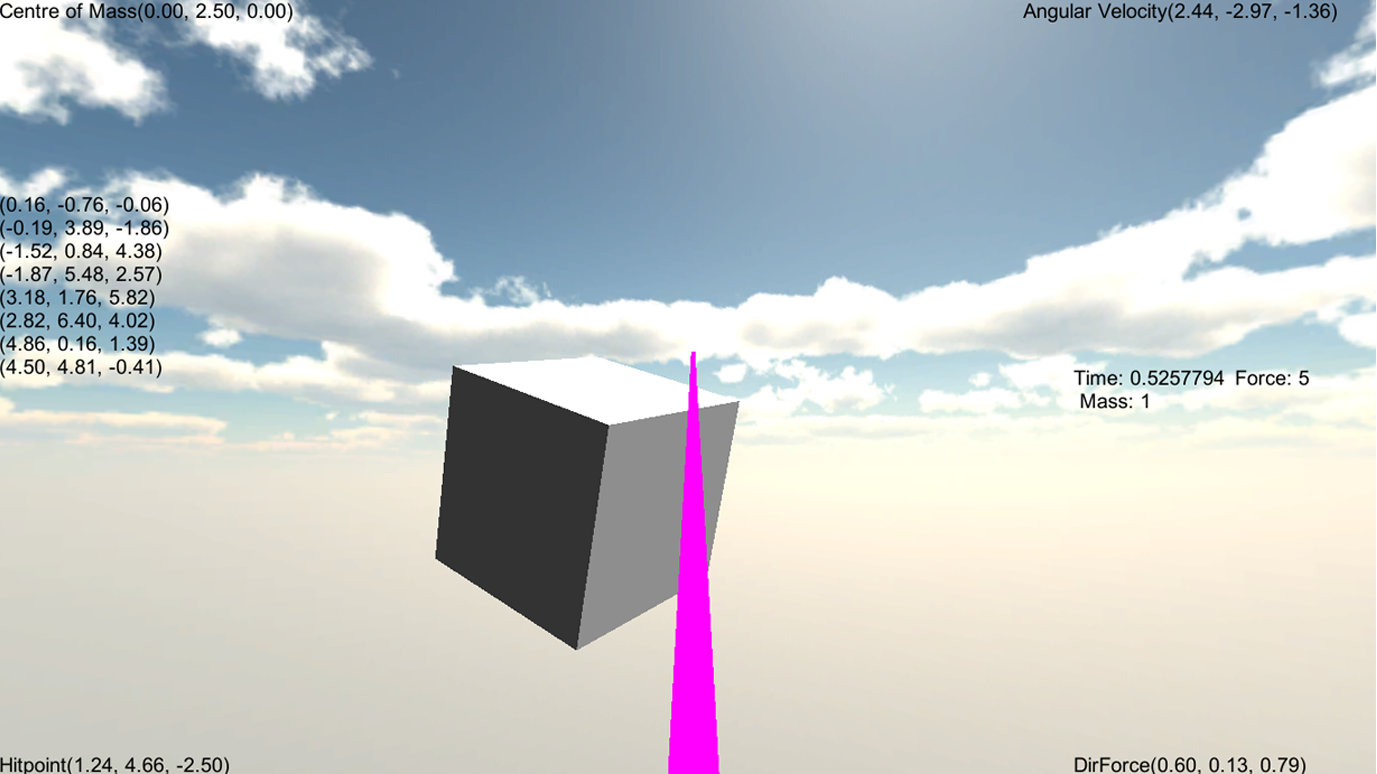
\includegraphics[width=\textwidth]{images/Screenshot2.PNG}
	\caption{Screenshot of Cube at $t = 0.526 s$}
	\label{fig:ScreenShotSingle}
\end{figure}

The equation going to be used to calculate the position b hand is equation \ref{eq:PositionGM} because in this scenario force is available meaning the acceleration can be worked out using Newton's Second Law $F=MA$.
\begin{equation}\label{eq:PositionGM}
\mathbf{p}=\frac{1}{2}\mathbf{A}t^{2}+{R}\tilde{\mathbf{p}_{0}}+\mathbf{g}
\end{equation}

For the hand calculation the angular velocity will be represented by $\boldsymbol{\omega}$ and will be taken from the application.
The force direction vector will also be taken form the application and will be represented by $F$.
Also shown in \ref{var:Rotation Variables} is $\mathbf{P}$ and this represents the initial position, and $\mathbf{g}$ which is the centre of mass.
Equations \ref{var:ftm} show three of the variables used $M$ being the mass of the object, $f$ is the force applied to the object, and $t$ is the time since the initial force has been applied. 
\begin{equation}\label{var:Rotation Variables}
	\boldsymbol{\omega} = 
	\begin{bmatrix}
		 2.44 \\
		-2.97 \\
		-1.36 
	\end{bmatrix}
	\qquad
	\mathbf{F} = f
	\begin{bmatrix}
		 0.6  \\
		 0.13 \\
		 0.79 
	\end{bmatrix}
	\qquad
	\mathbf{P}= 
	\begin{bmatrix}
		2.5 \\
		0 	 \\
		2.5 
	\end{bmatrix}
	\qquad
	\mathbf{g} = 
	\begin{bmatrix}
		0 \\
	 	2.5 	 \\
		0 
	\end{bmatrix}
\end{equation}
\begin{equation}\label{var:ftm}
	f = 5N
	\qquad
	t = 0.526s
	\qquad
	M = 1kg
\end{equation}
\begin{equation}\label{var:thetaomega}
	\omega = |\boldsymbol\omega| = 4.077
	\qquad
	\theta = \omega t = 2.144
\end{equation}
To start acceleration will have to be calculated this will be represented in calculations by $\mathbf{A}$.
It will be calculated as mentioned before using Newton’s Second Law $F=MA$.
This means in terms of this problem $\mathbf{A} = \mathbf{F}/M$ and we values are substituted in results in equation \ref{eq:Acceleration}.
\begin{equation}\label{eq:Acceleration}
	\mathbf{A} = \frac{f}{M}
	\begin{bmatrix}
		 0.6  \\
		 0.13 \\
		 0.79 
	\end{bmatrix} = 5
	\begin{bmatrix}
		 0.6  \\
		 0.13 \\
		 0.79 
	\end{bmatrix} = 
	\begin{bmatrix}
		 3  \\
		 0.65 \\
		 3.95 
	\end{bmatrix}
\end{equation}
Next $\tilde{\mathbf{p}_{0}}$ needs to be calculated, this is done by calculating the position vector of the point relative to the centre of mass,  $\mathbf{g}$, and can be shown in equation \ref{Eq:po}.
\begin{equation}\label{Eq:po}
	\tilde{\mathbf{p}_{0}} = \mathbf{P} - \mathbf{g} = 
	\begin{bmatrix}
		2.5 \\
		0 	 \\
		2.5 
	\end{bmatrix} -
	\begin{bmatrix}
		0 \\
	 	2.5 	 \\
		0 
	\end{bmatrix} =
	\begin{bmatrix}
		 2.5 \\
		-2.5 	 \\
		 2.5 
	\end{bmatrix}
\end{equation}
The next step is to calculate the matrix $R$, which is a standard rotational matrix about any axis.
Equation \ref{ma:GeneralRotation} is the initial matrix that will be used with $C$ being a shorthand for $(1-\cos\theta)$.
Below the rotational matrix are the values for $\alpha, \beta, \gamma$ in equation \ref{var:alphabetagamma} and in equation \ref{var:cs1-c} are the values of $\cos\theta, \sin\theta, (1-\cos\theta)$.
\begin{equation}\label{ma:GeneralRotation}
	R = 
	\begin{bmatrix}
		{\alpha}^{2}(C) + \cos\theta & 
		\alpha\beta(C) - \gamma\sin\theta & 
		\alpha\gamma(C) + \beta\sin\theta \\
		
		\alpha\beta(C) + \gamma\sin\theta & 
		{\beta}^{2}(C) + \cos\theta & 
		\beta\gamma(C) - \alpha\sin\theta \\
		
		\alpha\gamma(C) - \beta\sin\theta & 
		\beta\gamma(C) + \alpha\sin\theta & 
		{\gamma}^{2}(C) + \cos\theta \\
	\end{bmatrix}
\end{equation}
\begin{equation}\label{var:alphabetagamma}
	\alpha = \frac{\boldsymbol\omega_{x}}{\omega} = 0.5984
	\qquad
	\beta = \frac{\boldsymbol\omega_{y}}{\omega} = -0.7284
	\qquad
	\gamma = \frac{\boldsymbol\omega_{z}}{\omega} = -0.3336
\end{equation}
\begin{equation}\label{var:cs1-c}
	\cos\theta = -0.5421
	\qquad
	\sin\theta = 0.8403
	\qquad
	1-\cos\theta = 1.5421
\end{equation}
After substituting $\alpha, \beta, \gamma,\cos\theta, \sin\theta$, and $(1-\cos\theta)$ into the matrix the result can be seen in Matrix \ref{ma:Calculated Rotation}. Now multiply $R$ and $\tilde{\mathbf{p}_{0}}$ together in \ref{ma:CalculatedRPO} to get the vector $	R\tilde{\mathbf{p}_{0}} = (-1.29, -3.39, -2.36)$.
\begin{equation}\label{ma:Calculated Rotation}
	R = 
		\begin{bmatrix}
		   0.0102 & 
		  -0.3919 & 
		  -0.9199 \\
		  
		  -0.9525 & 
		   0.2761 & 
		  -0.1282 \\
		  
		   0.3043 & 
		   0.8776 & 
		  -0.3705 \\
	\end{bmatrix}
\end{equation}
\begin{equation}\label{ma:CalculatedRPO}
	R\tilde{\mathbf{p}_{0}} =
	\begin{bmatrix}
		  0.0102 & 
		  -0.3919 & 
		  -0.9199 \\
		  
		  -0.9525 & 
		  0.2761 & 
		  -0.1282 \\
		  
		  0.3043 & 
		  0.8776 & 
		  -0.3705 \\
	\end{bmatrix}
	\begin{bmatrix}
		 2.5 \\
		-2.5 	 \\
		 2.5 
	\end{bmatrix}
	= 
	\begin{bmatrix}
		 -1.2945 \\
		 -3.3921 \\
		 -2.3596 
	\end{bmatrix}
\end{equation}
$R\tilde{\mathbf{p}_{0}}$, $\mathbf{A}$, and $t^{2}$ can now be substituted back into equation \ref{eq:PositionGM} to find the final position of the chosen point.
\begin{equation}\label{eq:workout}
	\mathbf{p}=\frac{1}{2}
	\begin{bmatrix}
		 3  \\
		 0.65 \\
		 3.95 
	\end{bmatrix}
	0.526^{2}+
	\begin{bmatrix}
		 -1.2945 \\
		 -3.3921 \\
		 -2.3596 
	\end{bmatrix}
	+
	\begin{bmatrix}
	0 \\
	2.5 \\
	0
	\end{bmatrix}
\end{equation}
\begin{equation}\label{eq:working2}
	\mathbf{p}=
	\begin{bmatrix}
		 0.4145  \\
		 0.0898  \\
		 0.5158 
	\end{bmatrix}
	+
	\begin{bmatrix}
		-1.2945 \\
		-3.3921 \\
		-2.3596 
	\end{bmatrix}
	+
	\begin{bmatrix}
		 0 \\
		 2.5 \\
		 0 
	\end{bmatrix}
\end{equation}
\begin{equation}\label{eq:final}
	\mathbf{p}=
	\begin{bmatrix}
		-0.8801 \\
 		-0.8024 \\
 		-1.8138 
	\end{bmatrix}
\end{equation}

The final result for $\mathbf{p}$ is $(-0.88,-0.8,-1.81)$ and when compared to the application's vector of $(0.16,-0.76,-0.06)$ an error vector of $(1.04,0.04,1.75)$ can be calculated.
This vector is calculated by subtracting the calculated position vector from the applications position vector to show the difference between the two.

Using screenshots taking during the application, which can be seen in figure \ref{fig:ScreenShotFour}, more calculations can be done using all the same variables except for the time variable to see if the application is constantly different from the calculated result.
\begin{figure}[h]
	\centering
	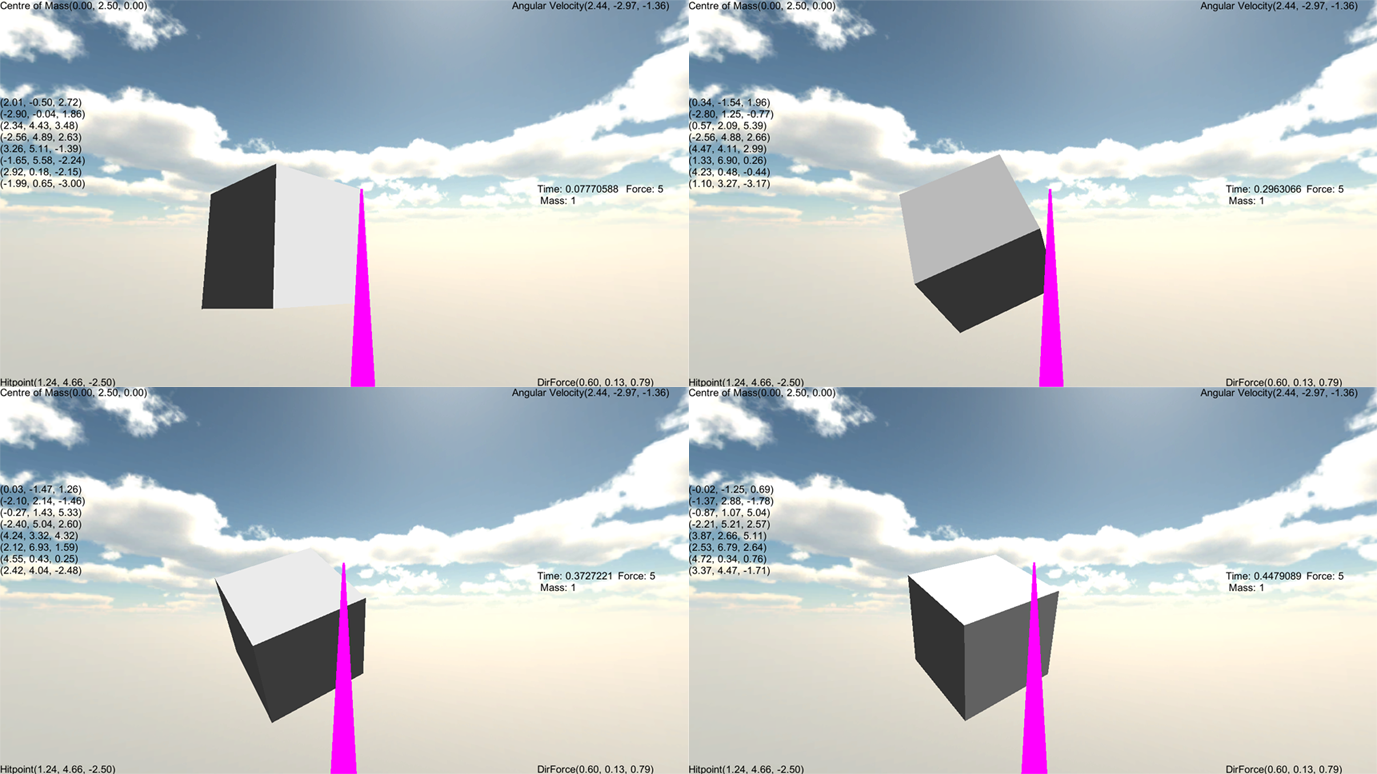
\includegraphics[width=0.8\textwidth]{images/Screenshot1.PNG}
	\caption{Screenshot of Cube at $t = 0.078 s$, $t = 0.296 s$, $t = 0.373 s$, $t = 0.498 s$}
	\label{fig:ScreenShotFour}
\end{figure}

The Table \ref{table:ErrorTable} shows the results from performing the previous calculations on different time steps both by hand and by the application.
Looking at the error vectors it can be seen that as the application continues the error between the application and the calculated results increase.
\begin{table}[h]
	\caption{Position Comparison}		% title of Table
	\centering							% used for centering table
	\begin{tabular}{c c c c}			% centered columns (4 columns)
		\hline\hline 					%inserts double horizontal lines
		$t$ (seconds) & Calculated Position & Application Position & Error Vector\\[0.5ex]% inserts table
		%heading
		\hline
		\centering								% inserts single horizontal line
		0.078 & $( 1.63,-0.69, 2.45)$ & $( 2.01,-0.50, 2.72)$ & $(0.38,0.19,0.27)$ \\
		0.296 & $(-0.50,-1.70, 0.83)$ & $( 0.34,-1.54, 1.96)$ & $(0.84,0.16,1.13)$ \\
		0.373 & $(-0.91,-1.62,-0.06)$ & $( 0.03,-1.47, 1.26)$ & $(0.94,0.16,1.32)$ \\
		0.448 & $(-1.04,-1.32,-0.96)$ & $(-0.02,-1.25, 0.69)$ & $(1.02,0.07,1.65)$ \\
		0.526 & $(-0.88,-0.80,-1.81)$ & $( 0.16,-0.76,-0.06)$ & $(1.04,0.04,1.75)$ \\ [1ex]	% [1ex] adds vertical space
		\hline									%inserts single line
	\end{tabular}
	\label{table:ErrorTable}					% is used to refer this table in the text
\end{table}

There could be a number of different reasons which have accumulated to give this error. For example it could be because of the way the physics engine in Unity3D handles rigid bodies but due to Unity3D being proprietary software it would be impossible to know exactly how the physics engine solves the problem or if any sacrifices where made to make performance fast and looking right compare to being actually physically realistic.
Also some of the errors could have come from rounding errors that follow through the equations, or from the possibility that the is timer not completely in sync with the physics engine in the application.